\subsubsection{Module 7: Hệ thống Thông báo (Notification)}
Hệ thống thông báo thời gian thực (Real-time) đóng vai trò then chốt trong việc giữ chân người dùng và đảm bảo thông tin mua bán được cập nhật tức thì.

\begin{figure}[H]
\centering
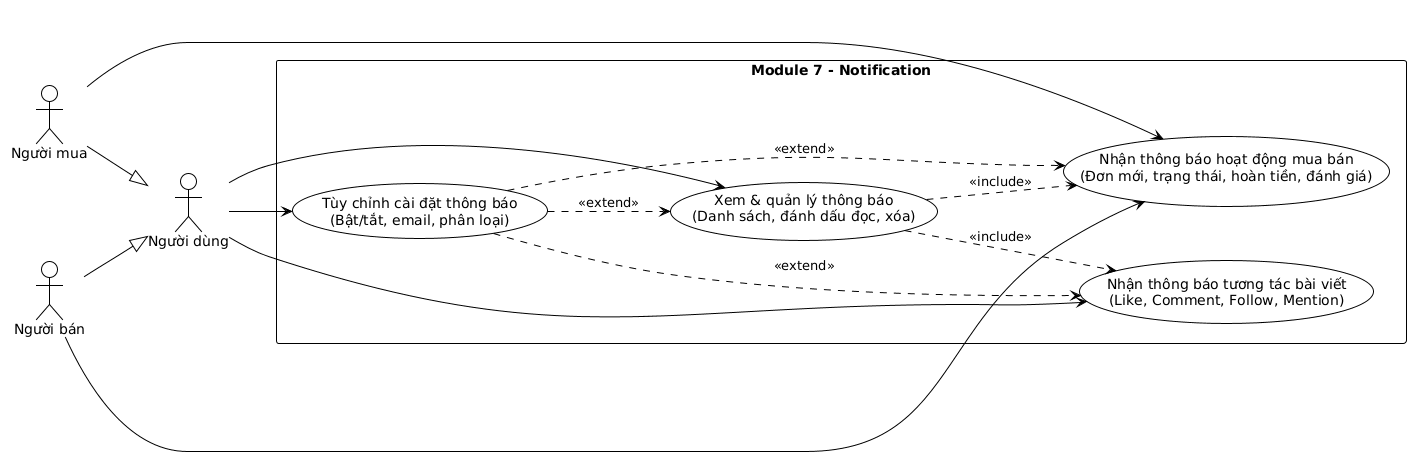
\includegraphics[width=\textwidth]{Images/Usecases/UC-M7-Notification.png}
\caption{Sơ đồ Use Case cho Module 7: Hệ thống Thông báo}
\label{fig:usecase-module7}
\end{figure}

\renewcommand{\arraystretch}{1.3}

% UC7.1: THÔNG BÁO TƯƠNG TÁC
\begin{table}[H]
\centering
\begin{tabularx}{\textwidth}{|l|X|}
\hline
\textbf{Tên Use Case} & \textbf{UC7.1: Nhận thông báo tương tác xã hội} \\ \hline
\textbf{Tác nhân} & Người dùng, Người bán \\ \hline
\textbf{Mô tả} & Hệ thống tự động gửi thông báo ngay lập tức đến người sở hữu bài viết khi có người khác thực hiện các hành động: thích bài viết, bình luận, theo dõi người dùng, hoặc được nhắc đến trong bình luận/bài viết của người khác. \\ \hline
\textbf{Kích hoạt} & Một người dùng khác thực hiện hành động tương tác với bài viết hoặc tài khoản của người nhận. \\ \hline
\textbf{Điều kiện tiên quyết} & 
\begin{itemize}
    \item Người nhận đã đăng nhập vào hệ thống ít nhất một lần trong phiên hiện tại.
    \item Người nhận không tắt hoàn toàn thông báo tương tác xã hội.
\end{itemize} \\ \hline
\textbf{Điều kiện sau} & 
\begin{itemize}
    \item Một thông báo mới xuất hiện trên giao diện người nhận.
    \item Số lượng thông báo chưa đọc tăng lên.
    \item Thông báo được lưu lại để người dùng có thể xem lại sau.
\end{itemize} \\ \hline
\textbf{Luồng sự kiện chính} & 
\begin{enumerate}
    \item Người dùng A thực hiện hành động (ví dụ: thích bài viết của Người dùng B).
    \item Hệ thống phát hiện hành động này.
    \item Hệ thống xác định chủ sở hữu bài viết (Người dùng B).
    \item Hệ thống tạo thông báo mới và gửi ngay lập tức đến Người dùng B.
    \item Giao diện của Người dùng B hiển thị thông báo.
    \item Người dùng B có thể nhấn vào thông báo để chuyển thẳng đến nội dung liên quan.
\end{enumerate} \\ \hline
\textbf{Luồng thay thế} & A1: Người dùng B đang không online $\rightarrow$ Thông báo vẫn được lưu và sẽ hiển thị ngay khi người đó đăng nhập lại. A2: Người dùng B tắt âm thanh thông báo $\rightarrow$ chỉ hiển thị hình ảnh. \\ \hline
\textbf{Ngoại lệ} & 
\begin{itemize}
    \item E1: Người dùng B đã chặn Người dùng A $\rightarrow$ Không gửi thông báo.
    \item E2: Bài viết ở chế độ riêng tư và Người dùng A không được phép xem $\rightarrow$ Không gửi thông báo.
\end{itemize} \\ \hline
\textbf{Ghi chú} & Tính năng quan trọng giúp tăng tính tương tác xã hội. \\ \hline
\end{tabularx}
\caption{Đặc tả Use Case Thông báo tương tác}
\end{table}

% UC7.2: THÔNG BÁO MUA BÁN
\begin{table}[H]
\centering
\begin{tabularx}{\textwidth}{|l|X|}
\hline
\textbf{Tên Use Case} & \textbf{UC7.2: Nhận thông báo hoạt động mua bán} \\ \hline
\textbf{Tác nhân} & Người mua, Người bán \\ \hline
\textbf{Mô tả} & Khi có sự kiện liên quan đến đơn hàng (đặt hàng mới, người bán xác nhận, giao hàng, hoàn thành, hủy đơn, yêu cầu hoàn tiền, có đánh giá mới…), hệ thống gửi thông báo ngay cho cả hai bên liên quan. \\ \hline
\textbf{Kích hoạt} & Bất kỳ thay đổi trạng thái nào của đơn hàng hoặc hành động liên quan đến đơn hàng. \\ \hline
\textbf{Điều kiện tiên quyết} & 
\begin{itemize}
    \item Người nhận có ít nhất một đơn hàng đang trong quá trình xử lý hoặc vừa hoàn tất.
    \item Người nhận chưa tắt thông báo liên quan đến mua bán.
\end{itemize} \\ \hline
\textbf{Điều kiện sau} & 
\begin{itemize}
    \item Cả người mua và người bán đều nhận được thông báo ngay lập tức.
    \item Thông báo chứa liên kết dẫn trực tiếp đến trang chi tiết đơn hàng.
\end{itemize} \\ \hline
\textbf{Luồng sự kiện chính} & 
\begin{enumerate}
    \item Người mua đặt một đơn hàng mới.
    \item Hệ thống tạo thông báo ``Bạn có đơn hàng mới'' gửi đến Người bán.
    \item Người bán xác nhận đơn hàng.
    \item Hệ thống gửi thông báo ``Đơn hàng của bạn đã được xác nhận'' cho Người mua.
    \item Tương tự với các trạng thái: đang giao, đã giao, hoàn thành, hủy, có đánh giá mới, có yêu cầu hoàn tiền…
\end{enumerate} \\ \hline
\textbf{Luồng thay thế} & A1: Một bên đang offline $\rightarrow$ Thông báo được lưu và hiển thị khi đăng nhập lại. A2: Có thể gửi thêm email nếu người dùng bật tùy chọn này. \\ \hline
\textbf{Ngoại lệ} & E1: Đơn hàng bị hủy ngay lập tức bởi người mua trước khi người bán nhìn thấy $\rightarrow$ chỉ gửi thông báo hủy. \\ \hline
\textbf{Ghi chú} & Tính năng này giúp người bán phản hồi nhanh đơn hàng và người mua luôn nắm được trạng thái mua sắm. \\ \hline
\end{tabularx}
\caption{Đặc tả Use Case Thông báo đơn hàng}
\end{table}

% UC7.3: QUẢN LÝ THÔNG BÁO
\begin{table}[H]
\centering
\begin{tabularx}{\textwidth}{|l|X|}
\hline
\textbf{Tên Use Case} & \textbf{UC7.3: Xem và quản lý danh sách thông báo} \\ \hline
\textbf{Tác nhân} & Người dùng \\ \hline
\textbf{Mô tả} & Người dùng có thể mở ra xem toàn bộ danh sách thông báo đã nhận (cả đã đọc và chưa đọc), đánh dấu đã đọc, hoặc xóa thông báo không còn cần thiết. \\ \hline
\textbf{Kích hoạt} & Người dùng nhấn vào biểu tượng chuông hoặc mục ``Thông báo'' trên thanh điều hướng. \\ \hline
\textbf{Điều kiện tiên quyết} & Người dùng đã đăng nhập và từng nhận ít nhất một thông báo. \\ \hline
\textbf{Điều kiện sau} & 
\begin{itemize}
    \item Danh sách thông báo được cập nhật trạng thái đọc/xóa theo hành động của người dùng.
    \item Số lượng thông báo chưa đọc giảm tương ứng.
\end{itemize} \\ \hline
\textbf{Luồng sự kiện chính} & 
\begin{enumerate}
    \item Người dùng nhấn vào biểu tượng thông báo.
    \item Hệ thống hiển thị danh sách tất cả thông báo (mới nhất ở trên).
    \item Thông báo chưa đọc được làm nổi bật.
    \item Người dùng có thể: Nhấn vào thông báo; Đánh dấu đã đọc; Xóa.
    \item Hệ thống cập nhật lại trạng thái và giao diện ngay lập tức.
\end{enumerate} \\ \hline
\textbf{Luồng thay thế} & A1: Người dùng chọn ``Xóa tất cả thông báo'' $\rightarrow$ toàn bộ thông báo bị xóa vĩnh viễn. \\ \hline
\textbf{Ngoại lệ} & E1: Không có thông báo nào $\rightarrow$ hiển thị dòng chữ ``Bạn chưa có thông báo nào''. \\ \hline
\textbf{Ghi chú} & Giao diện nên hỗ trợ phân loại thông báo để dễ theo dõi. \\ \hline
\end{tabularx}
\caption{Đặc tả Use Case Quản lý danh sách thông báo}
\end{table}

% UC7.4: CÀI ĐẶT THÔNG BÁO
\begin{table}[H]
\centering
\begin{tabularx}{\textwidth}{|l|X|}
\hline
\textbf{Tên Use Case} & \textbf{UC7.4: Tùy chỉnh cài đặt thông báo} \\ \hline
\textbf{Tác nhân} & Người dùng \\ \hline
\textbf{Mô tả} & Người dùng có thể tự quyết định sẽ nhận loại thông báo nào, qua kênh nào (trên web, âm thanh, email), và tắt hoàn toàn một số loại thông báo nếu muốn. \\ \hline
\textbf{Kích hoạt} & Người dùng vào phần Cài đặt $\rightarrow$ Thông báo. \\ \hline
\textbf{Điều kiện tiên quyết} & Người dùng đã đăng nhập. \\ \hline
\textbf{Điều kiện sau} & Cài đặt thông báo của người dùng được lưu lại và áp dụng cho mọi phiên đăng nhập sau này. \\ \hline
\textbf{Luồng sự kiện chính} & 
\begin{enumerate}
    \item Người dùng vào Trang cá nhân $\rightarrow$ Cài đặt $\rightarrow$ Thông báo.
    \item Hệ thống hiển thị danh sách các loại thông báo có thể bật/tắt.
    \item Người dùng bật/tắt từng mục và chọn có nhận qua email hay không.
    \item Người dùng nhấn ``Lưu cài đặt''.
    \item Hệ thống lưu và áp dụng ngay lập tức.
\end{enumerate} \\ \hline
\textbf{Luồng thay thế} & A1: Người dùng chọn ``Tắt tất cả thông báo'' $\rightarrow$ toàn bộ thông báo (trừ thông báo hệ thống bắt buộc) sẽ không hiển thị nữa. \\ \hline
\textbf{Ngoại lệ} & Không có. \\ \hline
\textbf{Ghi chú} & Tính năng này quan trọng để tránh làm phiền và tăng trải nghiệm cá nhân hóa. \\ \hline
\end{tabularx}
\caption{Đặc tả Use Case Cài đặt thông báo}
\end{table}